\chapter{The Execution Stack} \label{chp:the_execution_stack}

In this chapter we describe the execution stack. In section
\ref{sec:number_of_stacks} we'll look at the quantity and ownership of
execution stacks. Section \ref{sec:whats_on_the_stack} will examine the
entries of the stack, called stack frames. We'll see what data layout
a stack frame have to adhere to and look at some common stack
frames. Section \ref{sec:structure_of_stack} explains the structure of
the stack and how the convenient abstraction of the \texttt{Sp}-register
works.

The content in this chapter will stick to objective facts, mostly based
on the GHC source code. Difficulties of implementing stack traces will
be withheld for later chapters.

\section{Number of stacks} \label{sec:number_of_stacks}

Haskell's \texttt{base} library exports the following primitive \cite{base_forkIO}:
\mint{haskell}|forkIO :: IO() -> IO()|
Intuitively \texttt{forkIO} just creates another "green" thread running its argument.
Since there will be two concurrent threads running after this, clearly
another execution stack have been created somehow. In this section we
look at how many execution stacks there will be by looking at
where they are referenced from.

The implementation of \texttt{forkIO} is
that it will create another \emph{Thread State Object} (TSO). As
can be seen from figure \ref{fig:tso_definition}, a TSO points at a
Stack object fully reproduced in figure \ref{fig:stack_definition}.
Thread State Objects themselves are usually referenced from \emph{Capabilities}.
A Capability contains all essential values for executing
Haskell code. It can be thought as a virtual CPU, it contains
the virtual register values of the STG abstract machine. A capability also contains
a singly-linked deque of all TSOs that are scheduled to run, meaning
there is a one to many relationship between a capability and an execution
stack. Capabilities themselves also come in multitude in the run time
system (with the default settings). The number of
capabilities is configurable through a runtime option, as a rule of
thumb it should be set to as many as the number of cores on the computer
\cite{commentary_capabilities}. Figure \ref{fig:stacks} shows an example
of all the capabilities and TSOs at a particular moment of a running
Haskell program. The number of threads is dynamic of course, since
new threads can get created with \texttt{forkIO} and existing threads
can finish executing. Since GHC 7.6.1, the number of capabilities is
dynamic too \cite{haskell_org_release_7.6.1}.

In conclusion, there is one execution stack for each green thread (TSO).

\begin{figure}
\begin{mdframed}
  \begin{minted}{c}
typedef struct StgTSO_ {
    StgHeader               header;
    // deleted lines ...
    struct StgStack_       *stackobj;
    // ...
    struct Capability_*     cap;
    // ...
    StgWord32  tot_stack_size;
} *StgTSOPtr;
  \end{minted}
  \caption{The definition of \texttt{StgTSO} from the GHC run-time system
code}
  \label{fig:tso_definition}
\end{mdframed}
\end{figure}

\begin{figure}
\begin{mdframed}
  \begin{minted}{c}
typedef struct StgStack_ {
    StgHeader  header;
    StgWord32  stack_size;     // stack size in *words*
    StgWord32  dirty;          // non-zero => dirty
    StgPtr     sp;             // current stack pointer
    StgWord    stack[FLEXIBLE_ARRAY];
} StgStack;
  \end{minted}
  \caption{The definition of \texttt{StgStack} from the GHC run-time system
code}
  \label{fig:stack_definition}
\end{mdframed}
\end{figure}

\begin{figure}
\begin{mdframed}
  \centering
  \includegraphics[width=3.0in]{build/fig/stacks}
  \caption{Two virtual CPUs (Capabilities) running a total of three
green threads. Each green thread has its own execution stack.}
  \label{fig:stacks}
\end{mdframed}
\end{figure}

\section{What's on the Stack?} \label{sec:whats_on_the_stack}

In STG-land, all heap object have the layout shown in figure
\ref{fig:heap_object} \cite{commentary_heap_objects}.
A \emph{stack frame} is a heap object whose
info table's type is any of the types listed in figure \ref{fig:stack_types}.

\begin{figure}
\begin{mdframed}
  \centering
  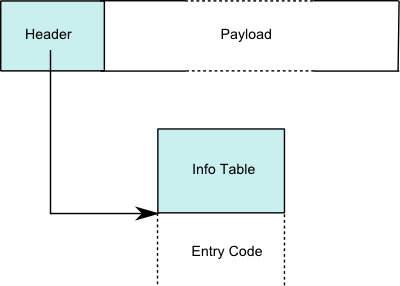
\includegraphics[width=3.0in]{fig/heap-object}
  \caption{Structure of heap objects in Haskell. TODO: Bilden är snodd!}
  \label{fig:heap_object}
\end{mdframed}
\end{figure}

\begin{figure}
\begin{mdframed}
  \begin{minted}{c}
#define RET_BCO                 31
#define RET_SMALL               32
#define RET_BIG                 33
#define RET_FUN                 34
#define UPDATE_FRAME            35
#define CATCH_FRAME             36
#define UNDERFLOW_FRAME         37
#define STOP_FRAME              38
// ... some omitted non-stack closure types ...
#define ATOMICALLY_FRAME        57
#define CATCH_RETRY_FRAME       58
#define CATCH_STM_FRAME         59
  \end{minted}
  \caption{The subset of closure types that are present on the stack.
The excerpt is from \cite{github_closure_types}. Which types that exist
on the stack is based on \cite{github_scavenge_stack}.}
  \label{fig:stack_types}
\end{mdframed}
\end{figure}


In this section we'll dive into
some details about the stack frames. Other details
are omitted, like how garbage collection is treating the closures.

\subsection{Fields and arguments}

We are used to think of the \emph{arity} of a function as the number
of \emph{arguments} that it takes. That is valid in the context
of the STG-machine \cite{commentary_function_calls}. But the arity
of the STG-function does not always equal with the number of times
a Haskell function can be applied to. Figure \ref{fig:tricky_arity}
shows one Haskell function which can be applied two arguments, but
is compiled to an STG-function with an arify of one.

\begin{figure}
\begin{mdframed}
        \begin{subfigure}[t]{0.5\textwidth}
          \begin{minted}{haskell}
f :: Bool -> Bool -> Bool
f = \x -> if x then not else id
          \end{minted}
          \caption{Haskell function}
        \end{subfigure}
    ~ %add desired spacing between images, e. g. ~, \quad, \qquad etc.
    %(or a blank line to force the subfigure onto a new line)
        \begin{subfigure}[t]{0.5\textwidth}
          \begin{minted}{haskell}
f = FUN(x -> case x of {
               True  -> not;
               False -> id });
          \end{minted}
          \caption{STG function, note that the number of arguments is
explicitly just one}
        \end{subfigure}
  \caption{In Haskell-land, the function can be fed up to two arguments.
  But we say that the arity is one, because the STG function that will be
  compiled takes one argument and returns a \texttt{FUN}. Note that \texttt{not}
  and \texttt{id} are themselves \texttt{FUN}s.
 }
  \label{fig:tricky_arity}
\end{mdframed}
\end{figure}

The return convention in the Cmm IR is to jump to the code of the
topmost stack frame \cite{commentary_return_convention}. If the code
take arguments, they are pushed on the stack before jumping to the
code. In addition to arguments, there are \emph{fields} too. Fields are
similar to arguments but are already placed on the stack and are part of
the stack frame. When a function is entered, the arguments are above the
info pointer field and the fields are below \cite{github_stack_at_call}, like
shown in figure \ref{fig:stack_at_call}. As an optimization some of the
arguments will be passed by the available registers of the virtual CPU,
the exact number of arguments that are passed by register will depend on
the backend that is targeted \cite{github_mach_regs_h}.

Figure \ref{fig:field_and_arguments} shows examples of Haskell code
that compile to code that has both fields and arguments. As soon will
be revelead in the next section, \texttt{case} expressions will be
splitting points in the code generation. The pre-\texttt{case} code will
push the post-\texttt{case} code on the stack. The post-\texttt{case}
code is also called a \emph{case continuation}. In order to not loose
the variables when evaluating the scrutiny, the live variables from
the pre-\texttt{case} code will be pushed along as the fields of the
post-\texttt{case} code. Jointly they form the \emph{case continuation
frame}. When a variable is not be needed by the case continuation, it
will not be a field, like in figure \ref{fig:no_fields}.

\begin{figure}
\begin{mdframed}
  \includegraphics[width=3in]{build/fig/stack_at_call}
  \caption{The stack when the topmost function on the stack is invoked .
In this case we pass the first argument by register, so \texttt{arg 1}
is stored in the virtual register \texttt{R1} described in the STG.}
  \label{fig:stack_at_call}
\end{mdframed}
\end{figure}

\begin{figure}
\begin{mdframed}
        \begin{subfigure}[t]{0.5\textwidth}
          \begin{minted}{haskell}
... = \x y -> ... case x of
                   4 -> x + y
                   _ -> x - y
          \end{minted}
          \caption{The case continuation will have \texttt{y} as a field
and \texttt{x} as an argument}
        \end{subfigure}
    ~ %add desired spacing between images, e. g. ~, \quad, \qquad etc.
    %(or a blank line to force the subfigure onto a new line)
        \begin{subfigure}[t]{0.5\textwidth}
          \begin{minted}{haskell}
... = \x y -> ... case x of
                   4 -> x + 5
                   _ -> x + 10
          \end{minted}
          \caption{The case continuation doesn't depend on \texttt{y}, so it
            will have no fields and \texttt{x} as its only argument.}
          \label{fig:no_fields}
        \end{subfigure}
  \caption{Two examples of code that will be turned into case
continuations.}
  \label{fig:field_and_arguments}
\end{mdframed}
\end{figure}

\subsection{The members of the stack} \label{sec:members_of_stack}

% TODO: "by their code" is hard to understand

Previously we defined what a stack frame is and enumerated
its types. However stack frames can also be categorized by their
code rather than their type. In this
section we look at stack frames, categorized by what they do.

\subsubsection{Case continuation frames}

Case continuations is what comes naturally from having lazy evaluation
in conjunction with pattern matching. When evaluating a case-expression, the code first
pushes the case continuation frame \emph{(\texttt{case} $\bullet$ \texttt{of}
\dots)} and then jumps to the entry code of the scrutiny. When the
scrutiny code returns, the code of the case continuation will have
that value as argument. Since that value is evaluated by now, it is
possible to have a C language style \texttt{switch-case} statement
corresponding to the original Haskell \texttt{case} statement,
or at least corresponding to the STG \texttt{case} statement.

\subsubsection{Update frames}

Consider the following code:

\begin{minted}[gobble=2]{haskell}
  let x = 2 + 3
  in x + x
\end{minted}

Here, \texttt{x} will only be evaluated once. This is implemented
through update frames. Update frames \emph{(Upd $\bullet$ \texttt{t})}
are pushed when a \texttt{THUNK \emph{x}} is evaluated, the frame's only
field will be the thunk itself \cite{github_thunk_code}. After the frame is
pushed, the entry code for \texttt{x} is entered. When the code returns,
the result is passed to the update frame as an argument, which will
overwrite the thunk with an indirection to its argument (the result of
\texttt{x}) \cite{github_updates_indirection}.


\subsubsection{Call continuation frames}

When evaluating \mint{haskell}|f True False|
where \texttt{f} is from figure \ref{fig:tricky_arity}, we have the
following scenario:

\begin{itemize}
  \item
    The function \texttt{f} has arity 1.
  \item
    We have an application of 2 arguments.
  \item
    The code has already type checked. We assume there is no
programming error and that \texttt{f True} will return another function.
\end{itemize}

We can't just jump to the code of \texttt{f} and forget about the last
argument \texttt{False}. Instead, we first put a call continuation
frame \emph{($\bullet$ \texttt{False})} and then jump to the code of \texttt{f}
\cite{evalapplyjfp06}.
When evaluation of \texttt{f True} is complete it returns to
the entry code of the call continuation, the call continuation would
first put its fields (\texttt{False}) on the stack (or write to
register \texttt{R1}) and then jump to the entry code of the argument it
got passed (the result of \texttt{f True}).
All call continuations are of closure type \texttt{RET\_SMALL}
\cite{github_genapply_RET_SMALL}.

\subsubsection{Underflow frames}

Underflow frames allow the stack itself to dynamically grow or
shrink. Their significance is discussed in section \ref{sec:structure_of_stack}.

\subsubsection{Other frames}

Figure \ref{fig:stack_types} showed that there are other closure types
that play a role on the Haskell execution stack, including retry frames
for Software Transactional Memory. We will not examine these other
frames further.

\section{Structure} \label{sec:structure_of_stack}

Since version 7.2.1, GHC switched its underlying structure of the
execution stack to use a chunked singly linked list rather than a
dynamically growing array
\cite{ghc_blog_overhaul_of_stack_management, ghc_changeset_stack_chunks}. When the stack chunk that
\texttt{tso->stackobj} is referencing gets full, it \emph{overflows},
then a new stack chunk is created with a reference to the first stack
and \texttt{tso->stackobj} is set to the new stack. Conversely, when
a stack chunk gets depleted, it \emph{underflows}, then we just
set \texttt{tso->stackobj} to point to what the underflow frame is
referencing, the garbage collector will later remove the abandoned
chunk. Figure \ref{fig:stack_structure} shows one execution stack
owned by a TSO whose stack has two chunks, hence it must have exactly
one underflow frame.

\begin{figure}
\begin{mdframed}
  \includegraphics[width=5in]{build/fig/stack_structure}
  \caption{Structure of the stack. The TSO is pointing at the current
  chunk and the older chunks are referenced by underflow frames.}
  \label{fig:stack_structure}
\end{mdframed}
\end{figure}

\subsection{Current stack pointer}

Each stack chunk is represented by the \texttt{StgStack}-struct
which has a member \texttt{sp} which is a stack pointer.
Since the execution stack is the collection of these chunks the
execution stack has multiple stack pointers. What the stack
pointers more exactly are pointing at is illustrated in figure
\ref{fig:stack_pointers}. But the only relevant stack pointer is what
we call the \emph{current stack pointer}, which is the one pointed by
\texttt{CurrentTSO->stackobj->sp}. \texttt{CurrentTSO} is a STG virtual
register. In C-land, the \texttt{CurrentTSO} virtual register is stored
in \texttt{cap->r->rCurrentTSO}, where \texttt{cap} is the Capability
that contains the \texttt{CurrentTSO} register. So there is one current
stack pointer for each Capability.

\begin{figure}
\begin{mdframed}
  \includegraphics[width=5in]{build/fig/stack_pointers}
  \caption{Demonstration of where the stack pointers are pointing}
  \label{fig:stack_pointers}
\end{mdframed}
\end{figure}

\subsubsection{Syncing}

The virtual CPU has the register \texttt{Sp} which also is a stack
pointer. \texttt{Sp} should be safe to assume to be in sync with
the current stack pointer. To make this so, whenever one jumps
from Cmm-land to C-land (from virtual CPU to real CPU), or vice
verse, it syncs. The exception is when it is not necessary, then there
is no syncing due to its overhead. Syncing does happen however on stack
underflows \cite{github_underflow_frame}. Note that while there is a
syncing between the virtual register \texttt{Sp} and the memory location
\texttt{CurrentTSO->stackobj->sp} \cite{github_sync_sp}, it also happens
for all the other virtual registers.

\subsection{Buffering}

Each time an overflow happens, there is some overhead. In the worst
case, a long alternating sequence of pushing and popping will cause
perpetual over and underflows. \emph{Buffering} is implemented to combat this,
buffering will copy a few frames from the old chunk to the new chunk
\cite{github_stack_buffering}, requiring that more than one frame have
to be popped before an underflow will happen.

\subsection{Stack squeezing}

When control is passed to an update frame, it will update its thunk and
then pass control to the next frame on the stack. An interesting scenario
is when there are consecutive update frames on the stack. In this case
all the consecutive update frames will be passed the exact same value
and will modify their respective thunks to an indirection to the same result.
\emph{Stack squeezing}
is to detect this scenario and remove all but one remaining update frame
and instead turn the affected thunks into indirections pointing to the
thunk that the remaining update frame points to. One example
is shown in figure \ref{fig:stack_squeezing}. \cite{github_thread_paused}

\begin{figure}
\begin{mdframed}
  \begin{subfigure}[t]{0.5\textwidth}
    \includegraphics[width=2.8in]{build/fig/squeeze-before}
    \caption{Before squeezing}
  \end{subfigure}
        ~ %add desired spacing between images, e. g. ~, \quad, \qquad etc.
          %(or a blank line to force the subfigure onto a new line)
  \begin{subfigure}[t]{0.5\textwidth}
    \includegraphics[width=2.8in]{build/fig/squeeze-after}
    \caption{After squeezing}
  \end{subfigure}
  \caption{An illustration of stack squeezing.
  }\label{fig:stack_squeezing}
\end{mdframed}
\end{figure}

Stack squeezing happens on overflows and is only run on the current
stack chunk. If the overflow is successful the overflow gets cancelled
\cite{github_return_if_squeezed}.
